\chapter{Cahier des charges}
\section{Scénario}
Le scénario a été construit grâce au site Mockflow, il a plusieurs fois évolué en fonction des souhaits des clients et des différentes améliorations proposées au fur et à mesure de la programmation.
Voici la maquette de la fenêtre en partie locale :
\begin{figure}[h!]
	\centering
   	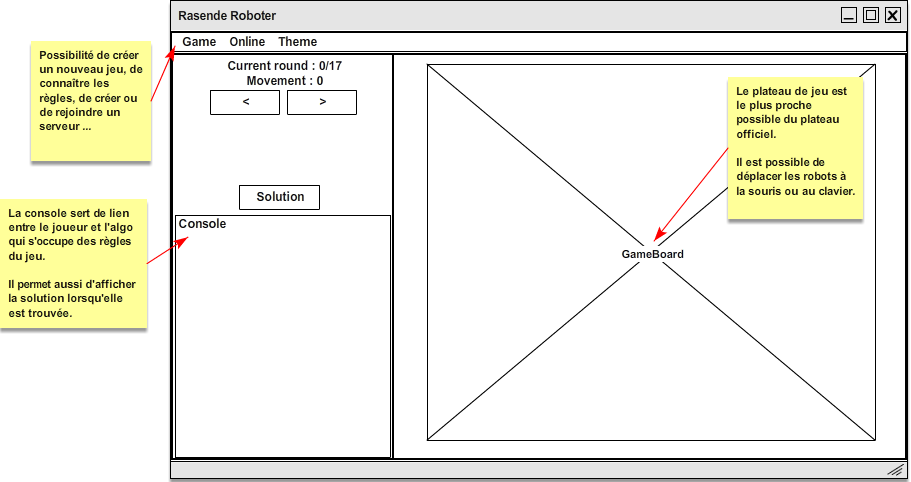
\includegraphics[scale=0.43]{img/local.png}
\end{figure}

L'interface se veut simple et épurée. Le joueur peut déplacer les robots sur le plateau soit à la souris soit avec le clavier pour aller plus vite. Le nombre de mouvement est automatiquement mis à jours jusqu'à ce qu'il atteigne la case objectif.
Si la partie se joue en ligne, de nouveaux éléments s'ajoutent à l'écran, comme la possibilité de proposer un nombre de mouvement ou la liste des joueurs connecté.
\newpage
\section{Besoins fonctionnels}
	\subsection{Jouer en local}
	La fenêtre de jeu en local est divisée en deux :
	\begin{itemize}
	\item A droite, le plateau de jeu.
	\item A gauche, une colonne qui contient :
		\begin{itemize}
		\item Les informations sur le jeu (numéro du tour, nombre de déplacements).
		\item Deux boutons permettant de revenir en arrière ou l'inverse pendant le jeu.
		\item Un bouton permettant de trouver la solution au tour.
		\item Une "console" qui affiche ce que doit faire le joueur à tout moment.
		\end{itemize}
	\end{itemize}

	Le menu de la fenêtre permet de commencer une nouvelle partie (avec un nouveau plateau construit aléatoirement en respectant les plateaux officiels), de quitter le jeu, d'afficher l'aide, de rejoindre ou de créer un serveur et de changer le thème du jeu.

	Spécificités de cet écran :
	\begin{itemize}
	\item Le premier couple de couleur de robot/emplacement à atteindre est défini (un nouveau couple sera redéfini à chaque nouveau tour de jeu).
	\item Déplacement à la souris ou au clavier pour résoudre la partie.
	\item Lorsque le joueur atteint l'objectif le tour est terminé, on choisit alors une nouvelle case objectif.
	\item Une fois les 17 tours terminés, la partie recommence.
	\end{itemize}

	\subsection{Jouer en ligne}
	
	Une partie en ligne débute en créant ou en rejoignant un serveur. Dans les deux cas, on se crée un profil rapide (en saisissant un nom de joueur). Le serveur synchronise tous les clients pour qu'ils aient le même plateau.

La fenêtre est similaire à celle du jeu en local. Cependant, le bouton solution est remplacé par : 
	\begin{itemize}
	\item[-] Un champ servant à proposer sa solution (le nombre de déplacement que l'on prévoit).
	\item Un encart avec la liste des joueurs et leur proposition respective.
	\item Un bouton pour déclarer forfait pendant un tour.
	\end{itemize}

	Spécificités de cet écran :
	\begin{itemize}
	\item Le joueur ne peut pas déplacer les robots, il doit trouver une solution dans sa tête.
	\item Une fois qu'un des joueurs a proposé sa solution, un compteur démarre. Pendant le décompte, chaque joueur peut proposer une proposition (meilleure ou non que la première). A la fin du temps, les joueurs sont classés en fonction de leur proposition. Celui qui a proposé le moins de mouvement prend la main.
	\item Le joueur qui a la main déplace les robots pour atteindre l'objectif. Il a autant de déplacements qu'il a proposé pour y arriver.
	\item Si le joueur ne retrouve pas la solution qu'il avait proposée il déclare forfait pour le tour et c'est le suivant dans le classement qui prend la main et ainsi de suite.
	\item Si personne ne trouve la solution, le tour est fini, on passe au suivant.
	\end{itemize}

	C'est le serveur qui s'occupe du bon fonctionnement de la partie, les clients ne récupèrent qu'une copie de la partie.

\section{Besoins non-fonctionnels}
\subsection{Jouabilité}
Le jeu doit être jouable, il est donc nécessaire d'avoir :
	\begin{itemize}
		\item une interface ergonomique et simple.
		\item des commandes intuitives, avec par exemple la possibilité d'utiliser les flèches pour le déplacement des robots et l'initiale de la couleur du robot pour en sélectionner un.
		\item un temps de réponse correct.
 	\end{itemize}

Il est également nécessaire pour garder un intérêt dans le jeu de tout faire pour éviter les possibilités de triche. Il faut notamment vérifier pendant les parties en réseau qu'il n'y a pas  de possibilité de tricher lorsqu'il y a un temps limite.

\subsection{Systèmes d'exploitation}
Le jeu doit être portable sur Linux et Mac. Pour cela, nous avons décidé de programmer le jeu en Java, plus précisément en Java 7 (il tourne donc aussi sous windows).

\subsection{Réutilisation}
Le choix d'une licence libre permettra au projet de continuer dans le temps et d'être repris. La mise en place d'une documentation (du type Javadoc) est aussi utile pour permettre au code d'être éventuellement modifié dans le futur.
Le code doit permettre une évolution rapide et facile en utilisant des Interfaces, en utilisant des noms de méthodes simples à comprendre, en permettant une lecture claire du code.

\section{Priorités}
	\begin{enumerate}
		\item Partie Solo.
		\item Algorithme trouvant la meilleure solution possible.
		\item Partie en réseau.
		\item En option : possibilité de construire son propre plateau de jeu.
		\item En option: nouvel algorithme plus "humain" permettant de faire des parties face à l'ordinateur en solo.
	\end{enumerate}

\section{Tableau des risques}
\begin{figure}[h!]
	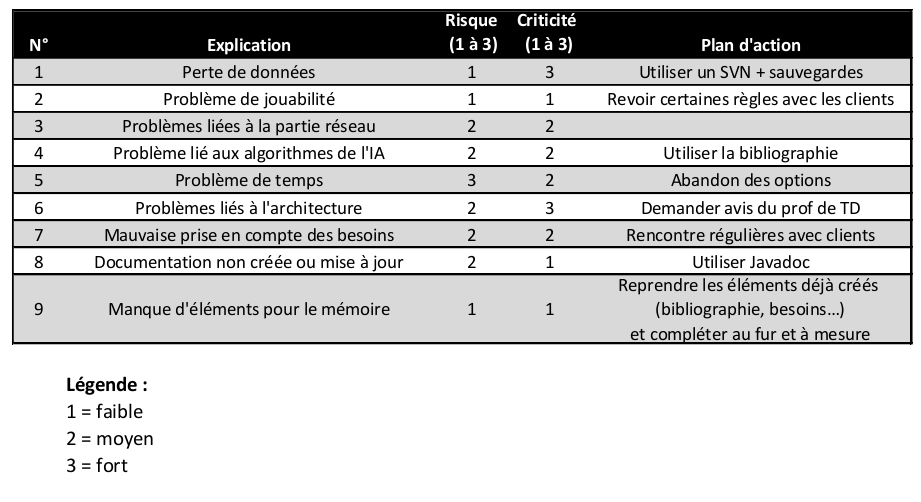
\includegraphics[scale=0.5]{img/risques.png}
\end{figure}
